\documentclass{beamer}

\usepackage{makecell}
\usepackage{dirtytalk}
\usepackage{hyperref}
\usepackage{listings}
\usepackage{color}
\definecolor{atomPurple}{RGB}{198,120,221}
\definecolor{atomRed}{RGB}{203,15,64}
\definecolor{atomGreen}{RGB}{0,128,0}
\definecolor{atomGreyLight}{RGB}{171,178,191}
\definecolor{atomGreyDark}{RGB}{92,99,112}
\definecolor{atomBlack}{RGB}{56,58,66}

\lstset{
language=C,
numbers=left,
showstringspaces=false,
tabsize=4,
columns=flexible,
keepspaces=true,
keywordstyle=\color{atomRed},
stringstyle=\color{atomGreen},
commentstyle=\color{atomGreyDark}
}

\title{Application Mapping for Network-on-Chip}
\author{Vaughan Kitchen}
\date{September 26, 2019}

\begin{document}

\begin{frame}
\titlepage
\end{frame}

\begin{frame}{Network-on-Chip}
	\begin{itemize}
		\item Topologies
			\begin{itemize}
				\item mesh
				\item torus
				\item octagon
				\item hypercube
				\item fat tree
				\item butterfly
				\item symmetric Clos
			\end{itemize}
		\item Routing
			\begin{itemize}
				\item Dimension-Ordered (DOR) / XY
				\item Valiant Load-Balancing (VAL)
				\item O1TURN
			\end{itemize}
		\item \textbf{Application Mapping}
			\begin{itemize}
				\item \textbf{NMAP}
				\item \textbf{LMAP}
				\item \textbf{PSMAP}
				\item \textbf{ILP}
			\end{itemize}
	\end{itemize}
\end{frame}

\defverbatim[colored]\lstchan{
\begin{lstlisting}
CHAN PickUp[4], PutDown[4], Enter[4], Exit[4] :
\end{lstlisting}
}

\defverbatim[colored]\lstphil{
\begin{lstlisting}
PROC Philosopher(VALUE identity) =
	WHILE TRUE
		SEQ
			Think
			Enter[identity]!ANY
			PickUp[identity]!ANY
			PickUp[identity+1 MOD 5]!ANY
			Eat
			PutDown[identity+1 MOD 5]!ANY
			PutDown[identity]!ANY
			Exit[identity]!ANY :
\end{lstlisting}
}

\defverbatim[colored]\lstforks{
\begin{lstlisting}
PROC Forks =
	VAR
		Free[4] :
	WHILE TRUE
		ALT i = [0 FOR 4]
			Free[i] & PickUp[i]?ANY
				Free[i] := FALSE
			PutDown[i]?ANY
				Free[i] := TRUE :
\end{lstlisting}
}

\defverbatim[colored]\lstroom{
\begin{lstlisting}
PROC Room =
	VAR
		Count :
	SEQ
		Count := 0
		WHILE TRUE
			ALT i = [0 FOR 4]
				Count<4 & Enter[i]?ANY
					Count := Count + 1
				Exit[i]?ANY
					Count := Count - 1 :
\end{lstlisting}
}

\defverbatim[colored]\lstmain{
\begin{lstlisting}
PAR
	Forks
	Room
	PAR i = [0 FOR 4]
		Philosopher(i)
\end{lstlisting}
}

\begin{frame}{Application Example - Dining Philosophers}
	\lstmain
	\lstphil
\end{frame}

\begin{frame}{Application Example - Dining Philosophers Continued}
	\lstroom
\end{frame}

\begin{frame}{Application Example - Dining Philosophers Continued}
	\lstforks
	\lstchan
\end{frame}

\begin{frame}{Network-on-Chip Mesh Example}
	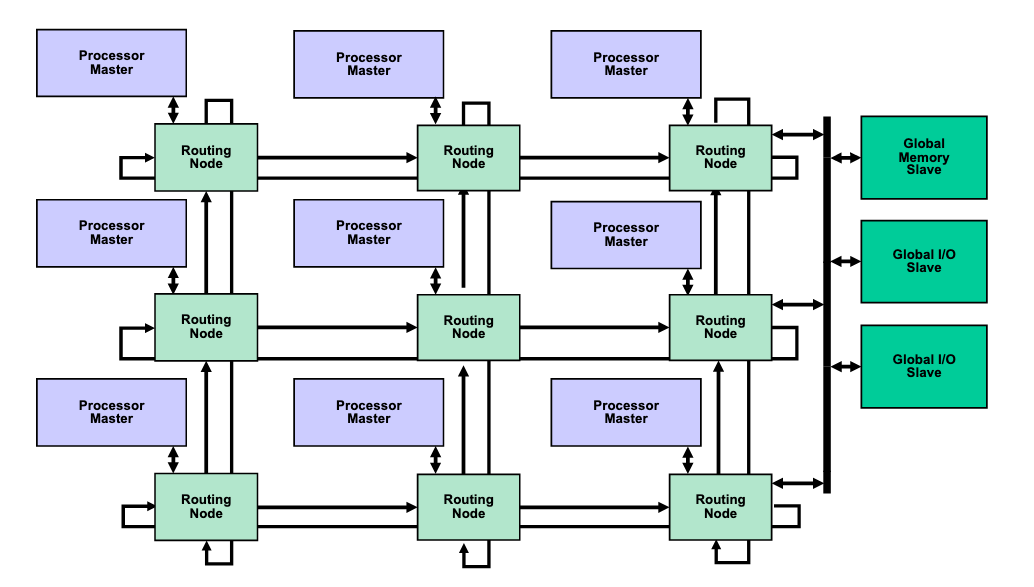
\includegraphics[width=\linewidth]{noc-mesh-example.png}
\end{frame}

\begin{frame}{Network-on-Chip Clos Example}
	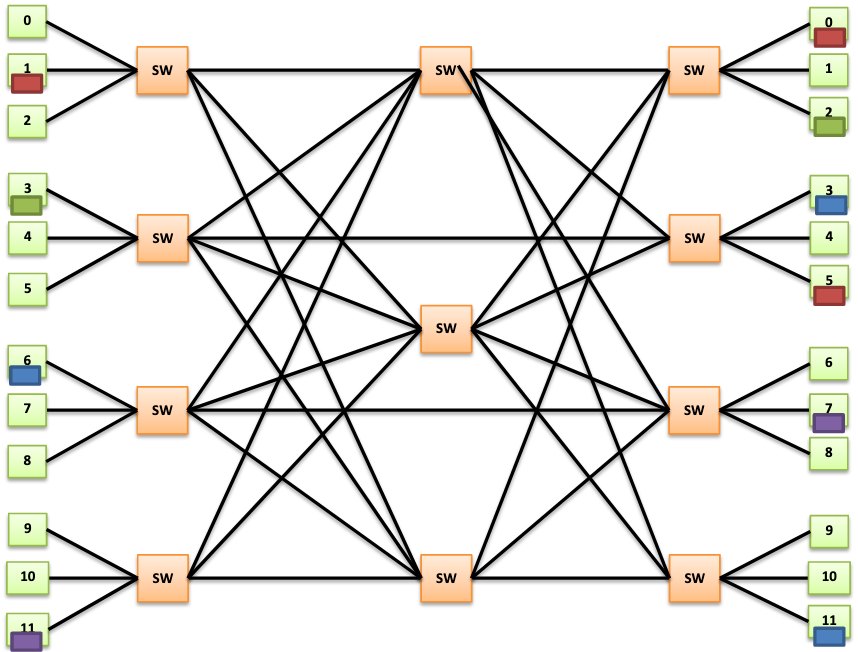
\includegraphics[width=\linewidth]{noc-clos-example.png}
\end{frame}

\begin{frame}{Application Graph Example}
	\begin{center}
		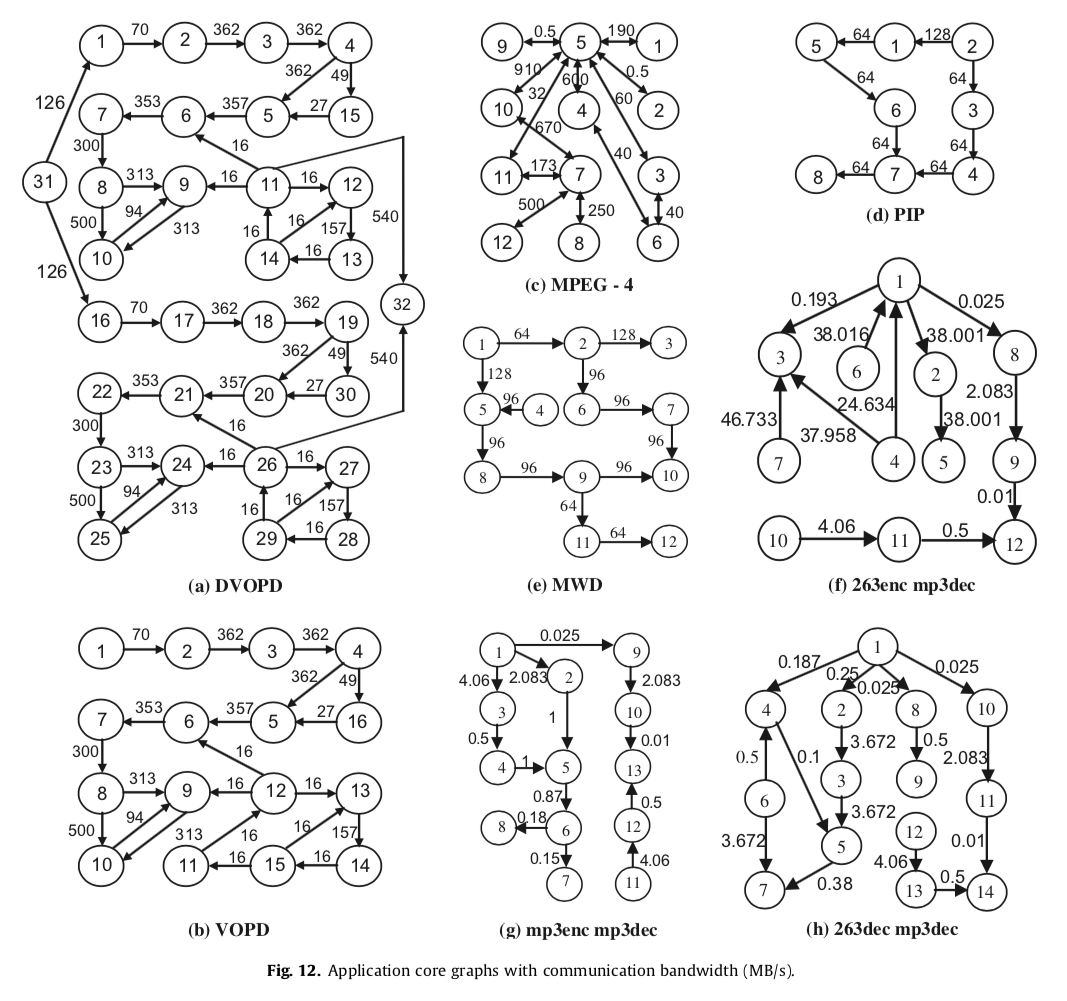
\includegraphics[width=0.8\linewidth]{application-graphs-example.png}
	\end{center}
\end{frame}

\begin{frame}{Application Graph Example Definitions}
	\begin{itemize}
		\item VOPD - Video Object Plane Decoding
		\item DVOPD - Dual Video Object Plane Decoding
		\item MWD - Multi-Window Displayer
		\item PIP - Picture-in-Picture
		\item MP3 - MPEG-1 Audio Layer III
		\item MPEG-4 - Moving Pictures Expert Group
	\end{itemize}
\end{frame}

\begin{frame}{Application Graph Example}
	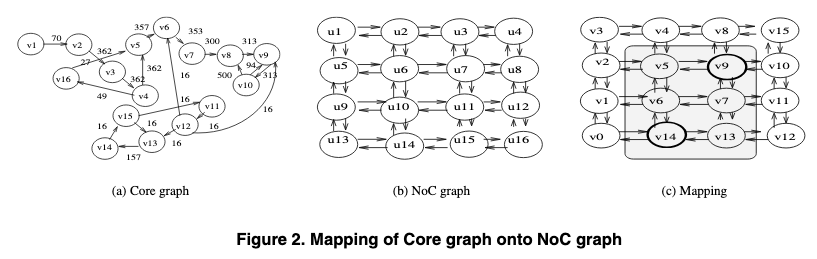
\includegraphics[width=\linewidth]{mapping-example.png}
\end{frame}

\begin{frame}{Problems}
	\begin{itemize}
		\item Nodes can have more than 4 connections
		\item Nodes can have uneven chain lengths (wrap?)
		\item More application nodes than hardware nodes
		\item Connections between early and late nodes
		\item Unbalanced cores or links (big.LITTLE)
		\item Mapping is NP-hard
		\item \textbf{What does the best mapping mean?}
	\end{itemize}
\end{frame}

\begin{frame}{Solution}
	\begin{center}
		\huge ad hoc topology
	\end{center}
\end{frame}

\begin{frame}{Actual solution}
	\begin{itemize}
		\item On-line mapping has too much overhead
		\item Use a static mapping algorithm
			\begin{itemize}
				\item NMAP - New Map? \\
					best performing at time of introduction
				\item LMAP - Kernighan-Lin (K-L) partitioning Map? \\
					performs better than NMAP
				\item PSMAP - Particle Swarm Map
				\item ILP - Integer Linear Programming \\
					optimal solution
				\item others
				\item (most algorithms only available for mesh networks)
			\end{itemize}
	\end{itemize}
\end{frame}

\begin{frame}{NMAP}
	\begin{enumerate}
		\item initial mapping
		\item minimum path computations
		\item repeat 2. with vertices pair-wise swapping
	\end{enumerate}
\end{frame}

\begin{frame}{NMAP - Continued}
	\textbf{Initial mapping}
	\begin{enumerate}
		\item the core with maximum communication placed onto maximally connected node
		\item repeatedly add unmapped cores with maximal communication to mapped cores
		\item place on node which minimizes cost with mapped cores (hop-count * bandwidth)
	\end{enumerate}
\end{frame}

\begin{frame}{NMAP - Continued}
	\textbf{Iterative improvement - minimum path}
	\begin{enumerate}
		\item form quadrant graph with source node in center
		\item destination node, and all nodes in shortest path will fall in one quadrant
		\item compute Dijkstra's shortest path algorithm using nodes of this quadrant paying attention to bandwidth in path computation
		\item repeatedly pairwise-swap and compute shortest path computations looking for a minima
	\end{enumerate}
\end{frame}

\begin{frame}{LMAP}
	\textbf{Initial mapping}
	\begin{enumerate}
		\item add dummy nodes if number of nodes is not a power of 2
		\item repeatedly perform K-L bi-partitioning (which calculates closeness of cores based on bandwidth)
		\item partitioning forms a hierarchical grouping of cores
		\item split the mesh in half alternating vertically and horizontally (bi-partitioning)
		\item allocate the cores to the nodes following the splits (most connected cores towards the centre)
	\end{enumerate}
\end{frame}

\begin{frame}{LMAP - Continued}
	\textbf{Iterative improvement}
	\begin{enumerate}
		\item for each partitioning level, partitioning is flipped and costs recomputed. the best cost is carried forward
		\item partitioning runs from strongest connected nodes outwards to the full node set
		\item once flipping completes dummy nodes are removed
	\end{enumerate}
\end{frame}

\begin{frame}{PSMAP}
	\begin{enumerate}
		\item performs Particle Swarm Optimization (PSO)
		\item nodes are numbered. cores randomly assigned to nodes for each initial particle
		\item local best (best the particle has seen), and global best saved each generation
		\item second generation is evolved by randomly swapping cores
		\item swap sequence considered as a series of swaps
		\item swap sequence to personal best, or global best applied with random probability
	\end{enumerate}
\end{frame}

\begin{frame}{ILP}
	\begin{itemize}
		\item Integer linear programming
		\item Formulated as 0-1 ILP
		\item Used Xpress-MP to solve
	\end{itemize}
\end{frame}

\begin{frame}{Algorithm Comparison}
	\begin{tabular}{c | r | r | r | r | r | r}
		\textbf{\thead{Mapping \\ algorithm}} & \multicolumn{2}{l |}{\textbf{VOPD}} & \multicolumn{2}{l |}{\textbf{MPEG-4}} & \multicolumn{2}{l |}{\textbf{PIP}}		\\
				&	\makecell{Comm. \\ cost} &	\makecell{CPU \\ in s.}	&	\makecell{Comm. \\ cost}	&	\makecell{CPU \\ in s.}	&	\makecell{Comm. \\ cost}	&	\makecell{CPU \\ in s.}	\\
		NMAP	&	4265.0	&	0.024	&	3672.0	&	0.016	&	640.0	&	0.010	\\
		LMAP	&	4189.0	&	0.040	&	4006.0	&	0.040	&	640.0	&	0.010	\\
		PSMAP	&	4119.0	&	0.260	&	3567.0	&	0.040	&	640.0	&	0.010	\\
		ILP		&	4119.0	&	4474.730	&	3567.0	&	21.530	&	640.0	&	1.280
	\end{tabular}
\end{frame}
	
\begingroup
\tiny
\begin{frame}{References}
	\begin{itemize}
		\item \url{http://prog.vub.ac.be/~tjdhondt/ESL/CSP_to_OCCAM_files/Section\%2013\%20-\%20CSP\%20to\%20OCCAM.pdf}
		\item \url{https://www.cs.otago.ac.nz/cosc402/lectures/lecture9.pdf}
		\item Pradip Kumar Sahu and Santanu Chattopadhyay. 2012. A survey on application mapping strategies for Network-on-Chip design. \url{http://dx.doi.org/10.1016/j.sysarc.2012.10.004}
		\item Sulyman Tosun et al. 2009. An ILP formulation for application mapping onto Network-on-Chips. \url{https://doi.org/10.1109/ICAICT.2009.5372524}
		\item Pradip Kumar Sahu et al. 2011. Application Mapping onto Mesh Structured Network-on-Chip using Particle Swarm Optimization. \url{https://doi.org/10.1109/ISVLSI.2011.21}
		\item Srinivasan Murali and Giovanni De Micheli. 2004. Bandwidth-Constrained Mapping of Cores onto NoC Architectures. \url{https://doi.org/10.1109/DATE.2004.1269002}
		\item Pradip Kumar Sahu et al. 2010. A New Application Mapping Algorithm for Mesh based Network-on-Chip Design. \url{https://doi.org/10.1109/INDCON.2010.5712700}
	\end{itemize}
\end{frame}
\endgroup

\begin{frame}{Questions?}
\end{frame}

\end{document}
